\documentclass[acmtog]{acmart}
\usepackage{graphicx}
\usepackage{subfigure}
\usepackage{natbib}
\usepackage{listings}
\usepackage{bm}

\definecolor{blve}{rgb}{0.3372549 , 0.61176471, 0.83921569}
\definecolor{gr33n}{rgb}{0.29019608, 0.7372549, 0.64705882}
\makeatletter
\lst@InstallKeywords k{class}{classstyle}\slshape{classstyle}{}ld
\makeatother
\lstset{language=C++,
	basicstyle=\ttfamily,
	keywordstyle=\color{blve}\ttfamily,
	stringstyle=\color{red}\ttfamily,
	commentstyle=\color{magenta}\ttfamily,
	morecomment=[l][\color{magenta}]{\#},
	classstyle = \bfseries\color{gr33n}, 
	tabsize=2,
	breaklines=true
}
\lstset{basicstyle=\ttfamily}

% Title portion
\title{Assignment 5:\\ {Rigid Body Simulation}}

\author{Name:\quad Yang Hongdi  \\ student number:\ 2019533234
\\email:\quad yanghd@shanghaitech.edu.cn}

% Document starts
\begin{document}
\maketitle

\vspace*{2 ex}

\section{Introduction}
In this assignment, simple rigid body simulation is performed without considering rotation. The intersection
between spheres and walls and intersection between spheres is performed.
\section{Implementation Details}
\subsection{Make the Scene Move}
To make the scene move, we update the spheres' P(linear momentum), speed and position every dt. As $$P = F * t = M * v$$
we update sphere's state by function below.
\begin{lstlisting}
void Sphere::Forward(float dt)
{
    for (Force const_force : constant_forces)
    {
        this->P += const_force.F * dt;
    }
    for (Force trans_force : transient_forces)
    {
        this->P += trans_force.F * dt;
    }
    this->v = this->P / this->M;
    this->x += this->v * dt;
    UpdateOpenGLObject();
}
\end{lstlisting}
\subsection{Collision Detect}
\subsubsection{SphereParallelgoram Collision Detection}
\quad For collision detection between sphere and parallelgoram, we first check the distance between sphere and the plane the parallelgoram is on.
\begin{lstlisting}
	vec3 normal = glm::normalize(glm::cross(parlgrm_s1, parlgrm_s2));
    vec3 temp_line = parlgrm_x - sphere_x;
    float dist = abs(glm::dot(normal, temp_line));

    if (dist - sphere_r > 0) // not intersect
    {
        collision_info.is_collided = false;
        return false;
    }
\end{lstlisting}
Then we will check if the intersect circle is in the parallelgoram. We first check if the collision point is in the parallelgoram, and then we will check
if the circle intersect with each edge of the parallelgoram.
\subsubsection{SphereSphere Collision Detection}
\quad For collision detection between spheres, we simply compute the distance between the center of spheres. If the distance is smaller than the sum of two spheres' radius, then
the two spheres are collided.
\subsection{Adjust Collision}
As we are updating the spheres' state discontinuously, it is possible that the sphere would collide with wall at a deep point in the wall, so the sphere may not be able to get out
next dt and then it will go into the wall. To prevent this, we need to adjust the collision.\\
To adjust the collision, we need to find a time between t and $t + \Delta t$ where the intersection degree is in the intersection tolerance.
\begin{figure}[H]
	\centering
	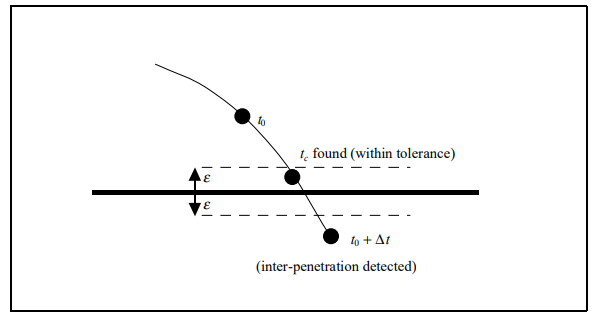
\includegraphics[width=3.2in, height = 2in]{images/interpenetration.png}
	\caption{find tc in tolerance}
\end{figure}
so we find the suitable time $t_c$ recursively between t and $t + \Delta t$.
\begin{lstlisting}
void Scene::FindRealCollision(float& intersect_degree, float delta_t)
{
    if (!IsCollided(intersect_degree))
    {
        this->Forward(delta_t / 2);
        return FindRealCollision(intersect_degree, delta_t / 2);
    }
    else if (intersect_degree - intersect_tolerance > 1e-4)
    {
        this->Backward(delta_t);
        this->Forward(delta_t / 2);
        return FindRealCollision(intersect_degree, delta_t / 2);
    }
}
\end{lstlisting}
\subsection{Handle Colliding contact}
\subsubsection{Handle collision between sphere and wall}
\quad When handling collison between sphere and wall, as wall is static, we consider its Mass as infinity and zero speed.\\
Then we compute the sphere's speed along the normal direction of the wall.
\begin{lstlisting}
	vec3 sphere_speed = sphere.GetV();
	vec3 normal = glm::normalize(sphere.GetX() - temp_collision_info.collision_point);
	float vrel = glm::dot(sphere_speed, normal);// relative speed on normal direction
	vec3 v_normal = vrel * normal;
\end{lstlisting}
If $v_{rel} > threshold$, we consider the ball is leaving the wall, thus not collided.\\
If $v_{rel} > -threshold$, we consider the ball has resting contact with the wall, and we will apply support force on the sphere.
\begin{lstlisting}
	Force sphere_press_force;
	for (Force force : sphere.constant_forces) sphere_press_force.F += force.F;
	for (Force force : sphere.transient_forces) sphere_press_force.F += force.F;
	sphere_press_force.F = glm::dot(sphere_press_force.F, normal) * normal;
	Force N;
	N.F = -sphere_press_force.F; // support force
\end{lstlisting}
And if neither of above, we do the real collision handling.\\
We consider the collision make the sphere's relative speed $v_{rel}$ become $-0.8 * v_{rel}$ in dt time, so we compute F by
$$F = \frac{M\cdot-(1+0.8)\cdot v_{rel}}{dt}$$
During collision, we also consider the speed will decrease 0.01 along the tangent direction, so we also add a Force $F = \frac{M\cdot-(1 - 0.99)\cdot v_{tan}}{dt}$
to the sphere.
\subsubsection{Handle collision between spheres}
\quad For the collision between spheres, we also first compute the relative speed along the intersection direction.
The relative speed is considered as $v_1 - v_2$
\begin{lstlisting}
	vec3 sphere1_speed = sphere1.GetV();
	vec3 sphere2_speed = sphere2.GetV();
	vec3 collision_normal = glm::normalize(sphere1.GetX() - sphere2.GetX());
	float vrel = glm::dot(sphere1_speed - sphere2_speed, collision_normal);
	vec3 v_normal = vrel * collision_normal;
\end{lstlisting}
Then, same as above, we check if the sphere is leaving each other or having resting contact.\\
If the spheres are having real collision, we consider the collision make the relative speed $v_{rel}$ become $-0.8 * v_{rel}$, and we compute the
total collision force F.
$$F = \frac{-(1+0.8)\cdot v_{rel}}{(\frac{1}{M_1} + \frac{1}{M_2})\cdot dt}$$
And for each ball, we add $\frac{F}{2}$ on it.\\
\\ The transient forces will be cleared immediately after updating the sphere for next dt.
\section{Results}
The results will be showed in real-time to TAs.
\newpage
\begin{figure}[H]
		\centering
		
		\subfigure[Scene0]{
		\begin{minipage}[t]{0.45\linewidth}
		\centering
		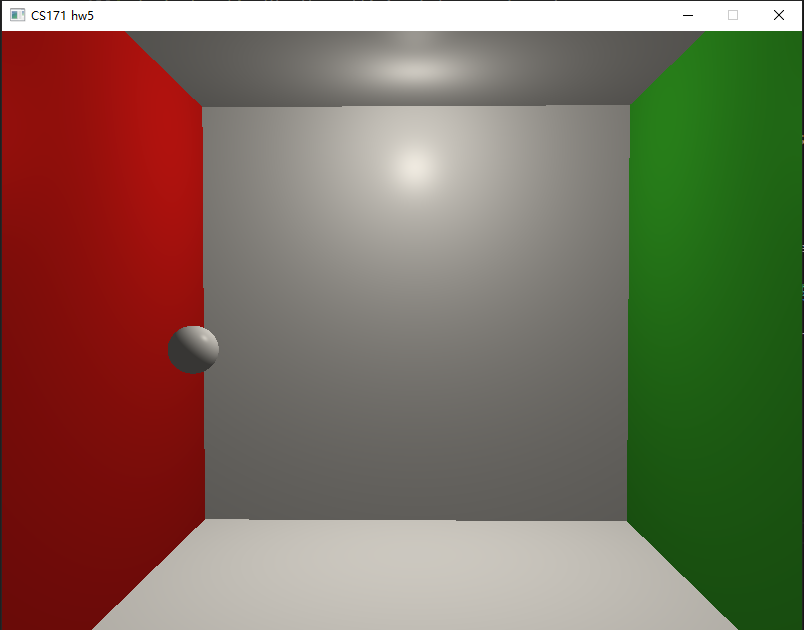
\includegraphics[width=2.5in]{images/scene0.png}
		%\caption{original image}
		\end{minipage}%
		}

		\subfigure[Scene1]{
		\begin{minipage}[t]{0.45\linewidth}
		\centering
		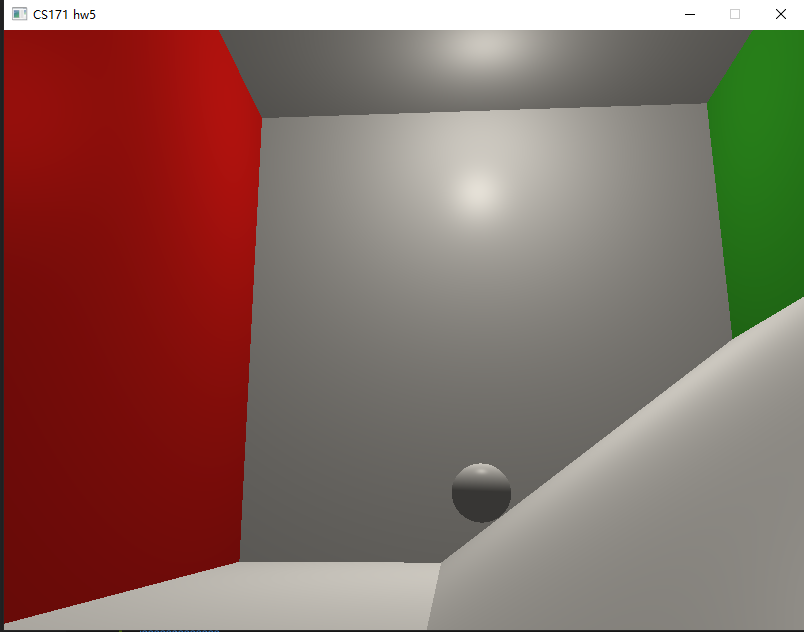
\includegraphics[width=2.5in]{images/scene1.png}
		%\caption{original image}
		\end{minipage}%
		}

		\subfigure[Scene2]{
		\begin{minipage}[t]{0.45\linewidth}
		\centering
		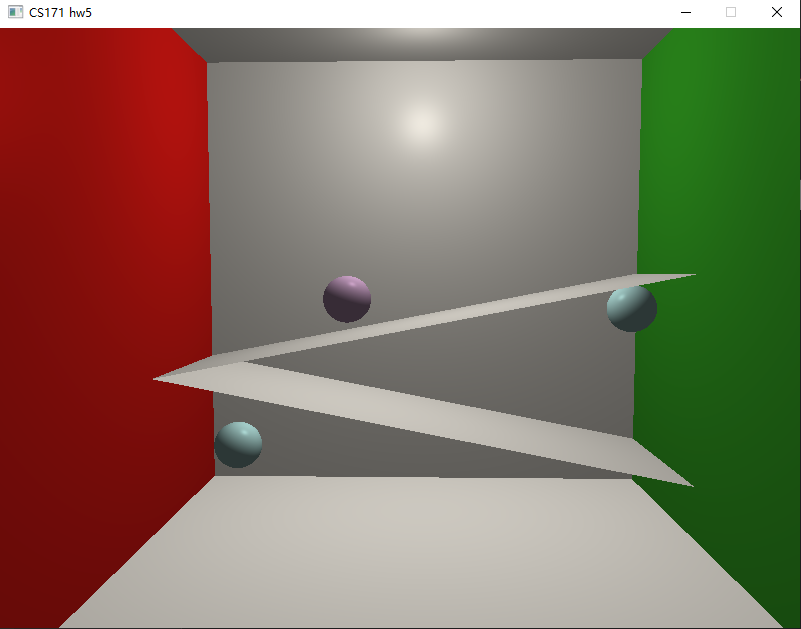
\includegraphics[width=2.5in]{images/scene2.png}
		%\caption{original image}
		\end{minipage}%
		}

		\subfigure[Scene3]{
		\begin{minipage}[t]{0.45\linewidth}
		\centering
		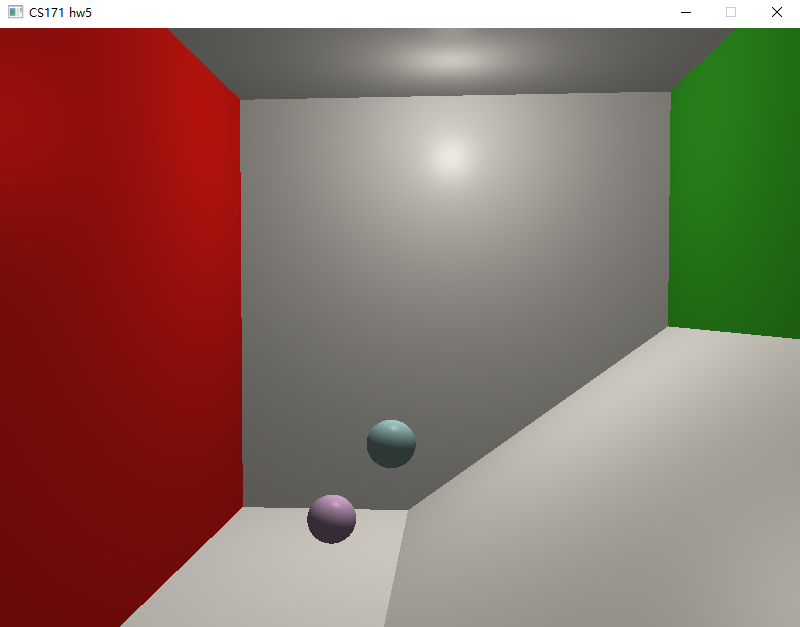
\includegraphics[width=2.5in]{images/scene3.png}
		%\caption{original image}
		\end{minipage}%
		}
	\end{figure}
	\begin{figure}[H]
		\centering
		\subfigure[Scene4]{
			\begin{minipage}[t]{0.45\linewidth}
			\centering
			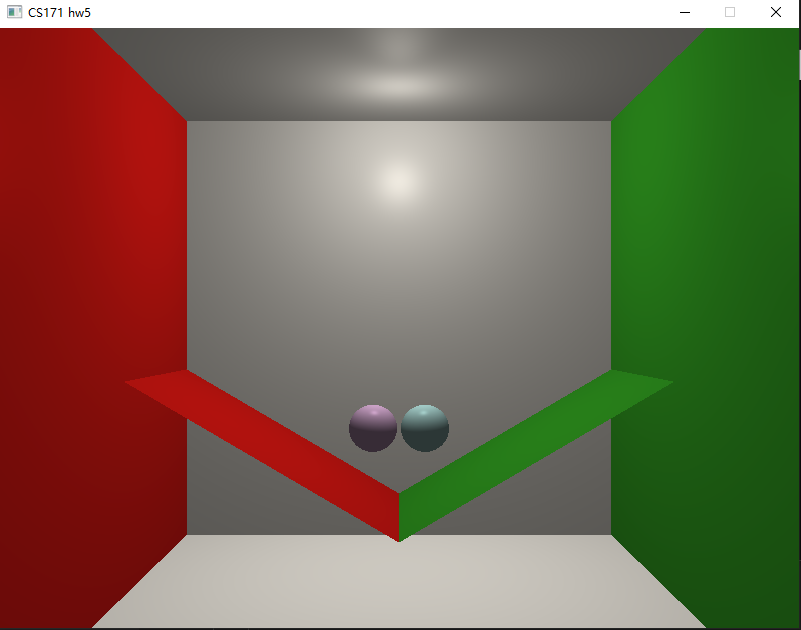
\includegraphics[width=2.5in]{images/scene4.png}
			%\caption{original image}
			\end{minipage}%
			}
	\end{figure}
\end{document}
